\section{State and Event Identity}
\label{sec:canonicalization}

Deduplication decides how large the explored set is: without it, every path to a state adds a separate vertex, and the number of paths grows super-exponentially when rewrites add edges. Two states are the same node when their hypergraphs are isomorphic, with vertex relabeling allowed and within-edge order and edge multiplicity preserved. The exact mode computes an individualization--refinement (IR) canonical form for every state and deduplicates by a 64-bit hash of that form, which two isomorphic states always share; two non-isomorphic states share it only through a hash collision, which the engine does not check for.

\subsection{Individualization--Refinement}
\label{sec:ir}

The canonical form is computed by McKay-style individualization--refinement~\cite{mckay2014practical}, the family of algorithms behind nauty and Traces. IR produces a canonical labeling, together with automorphism generators and vertex and edge orbits, such that two hypergraphs receive the same canonical form if and only if they are isomorphic.

\begin{definition}[Canonical Form]
A canonicalization $\canon$ maps each hypergraph to a labeled representative such that $\canon(\hypergraph_1) = \canon(\hypergraph_2)$ iff $\hypergraph_1 \cong \hypergraph_2$.
\end{definition}

IR refines a vertex coloring until it is stable. If a cell with more than one vertex remains, it \emph{individualizes} one of its vertices (gives it a unique color) and recurses, which produces a search tree of refinements. Automorphisms found during the search prune symmetric branches, and the lexicographically extremal leaf defines the canonical labeling.

\begin{remark}[Complexity]
Like nauty, IR is exponential in the worst case and polynomial in the state size on states without large automorphism groups. The worst case occurs on highly symmetric states, where the exact mode's cost is concentrated. Proposition~\ref{prop:wlceiling} bounds what a cheaper filter in front of IR can save.
\end{remark}

The automorphism generators and edge orbits from IR are used again for event canonicalization and for the exact reconstruction of causal and branchial multiplicities.

\paragraph{Search bounds.} The search has two bounds: the individualization depth and the number of automorphism generators recorded. Exceeding either is reported, and the engine raises the bound and runs the search again. The two fail differently. Reaching the depth bound before the coloring is discrete produces no canonical form, so the failure is visible. A full generator table still produces a correct canonical hash, but the orbits, which are built by fusing edges over the recorded generators, come out too fine. The quotient reconstruction identifies instances by these orbits (Section~\ref{sec:quotient}), so a truncated generator table would give a wrong result with no error. The generator bound is therefore raised on overflow in the same way as the depth bound. Raising the generator bound cannot fix a depth failure, so escalation stops at the first depth failure.

\paragraph{Symmetric states.} When a state has nontrivial automorphisms, IR selects one of several equivalent labelings by a tie-break within cells, and the tie-break depends on the order in which the state's vertices are numbered. Two numbering conventions give the same canonical hash but can assign different ranks to the same edge. Edge ranks identify consumed and produced edges across a rewrite, so one numbering convention is shared by every caller. On the equivalence probe's 4063-state corpus, encounter-order numbering and sorted-unique numbering assign different ranks on 103 states, all with nontrivial automorphisms.

\subsection{A Ceiling on Pre-Filters}
\label{sec:wl}

A sound invariant cheaper than IR, such as Weisfeiler--Leman color refinement~\cite{weisfeiler1968reduction,shervashidze2011weisfeiler}, could filter states before canonicalization: hash every state cheaply and run IR only when the cheap hash repeats. Proposition~\ref{prop:wlceiling} bounds the saving.

\begin{proposition}[Ceiling on a pre-filter]
\label{prop:wlceiling}
Let a run produce $R$ raw states falling into $C$ isomorphism classes, and let $f$ be a sound isomorphism invariant: isomorphic states receive equal $f$-values. Consider deduplication that computes $f$ on each raw state, and invokes IR only when the value has been seen before. Then the number of IR invocations is at least $R - C$, so the fraction of IR calls avoided is at most $C/R$, and one $f$-pass is paid on all $R$ states.
\end{proposition}

\begin{proof}
Soundness means states in one class share an $f$-value, so the number of distinct values is at most $C$. A state whose value is already present cannot be resolved by $f$: equal values are consistent both with isomorphism and with an $f$-collision, so IR is invoked. At most one state per distinct value finds its value absent, hence at most $C$ states skip IR and at least $R - C$ invoke IR.
\end{proof}

$C/R$ depends on the rule and the depth. Table~\ref{tab:crratio} and Figure~\ref{fig:crratio} give it for each corpus workload at two depths.

\begin{table}[htbp]
\centering
\caption{\textbf{Canonical classes as a fraction of raw states, per corpus workload.} $C/R$ is
the upper bound of Proposition~\ref{prop:wlceiling} on the fraction of IR calls a pre-filter can
skip. The event count is given beside it because a ratio from a small run is weaker evidence than
the same ratio from a large one.}
\label{tab:crratio}
% GENERATED by tools/dev/paper_tables.py -- do not edit.
% commit 1d5bc1c9 | Intel(R) Core(TM) i9-14900K, 20 GB RAM, Linux 5.15.167.4-microsoft-standard-WSL2 | source: tools/cost_matrix.cpp
\resizebox{\ifdim\width>\linewidth\linewidth\else\width\fi}{!}{%
\begin{tabular}{llrrr}
\toprule
Case & Rule type & Events & $C/R$ & $C/R$ at lower depth \\
\midrule
\texttt{cycle4-automorphic} & automorphism & 68{,}184 & 0\% & 12\% \\
\texttt{star4-automorphic} & automorphism & 68{,}184 & 0.3\% & 20\% \\
\texttt{disconnected-lhs} & disconnected & 126 & 0.8\% & 14.3\% \\
\texttt{binary-growth} & productive/arity2 & 873 & 4.1\% & 75\% \\
\texttt{multi-rule} & multi-rule & 237 & 15.1\% & 83.3\% \\
\texttt{triangle} & productive/mixed-conn & 124 & 28.8\% & 60\% \\
\texttt{arity3-growth} & arity3 & 153 & 42.2\% & 100\% \\
\texttt{self-loop} & self-loop/arity2 & 1 & 100\% & 100\% \\
\bottomrule
\end{tabular}
}

\end{table}

% GENERATED by tools/dev/paper_tables.py -- do not edit.
% commit 9fb1039 | measured on AMD EPYC 9174F 16-Core Processor, 503 GB RAM, Linux 6.8.0-138-generic | load at start 3.09/2.50 (1m/15m) | source: tools/cost_matrix.cpp

\pgfplotsset{crsymbolic/.style={symbolic x coords={cycle4,star4,disconn,binary,multi,triangle,arity3,self-loop}}}

\begin{figure}[tb]
\centering
\resizebox{\linewidth}{!}{%
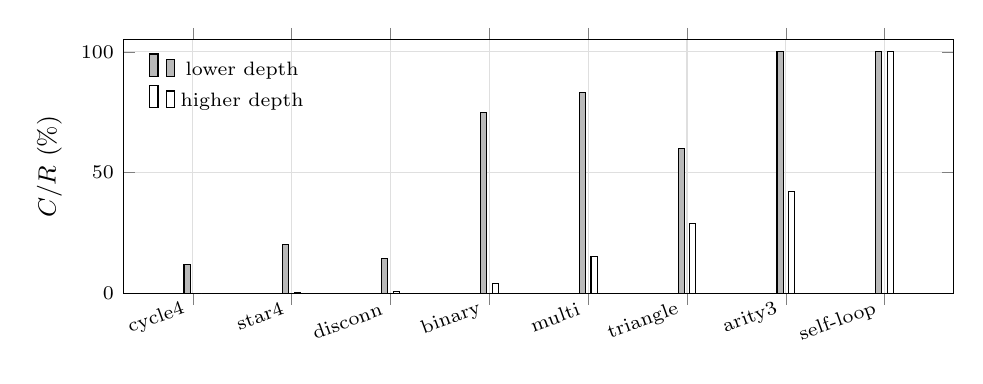
\begin{tikzpicture}
\begin{axis}[
    width=\linewidth, height=4.8cm,
    ybar, bar width=2.2pt,
    ylabel={$C/R$ (\%)}, ymin=0, ymax=105,
    crsymbolic,
    xtick=data, x tick label style={font=\scriptsize, rotate=20, anchor=east},
    grid=major, grid style={gray!25},
    legend style={font=\scriptsize, at={(0.02,0.97)}, anchor=north west, draw=none, fill=none},
    label style={font=\small}, tick label style={font=\scriptsize},
]
% GENERATED by tools/dev/paper_tables.py -- do not edit.
% commit 4f4af3d | measured on AMD EPYC 9174F 16-Core Processor, 503 GB RAM, Linux 6.8.0-138-generic | load at start 1.34/1.00 (1m/15m) | source: tools/cost_matrix.cpp

\addplot[fill=gray!55, draw=black] coordinates {(cycle4,12)(star4,20)(disconn,14.3)(binary,75)(multi,83.3)(triangle,60)(arity3,100)(self-loop,100)};
\addlegendentry{lower depth}
\addplot[fill=white, draw=black] coordinates {(cycle4,0)(star4,0.3)(disconn,0.8)(binary,4.1)(multi,15.1)(triangle,28.8)(arity3,42.2)(self-loop,100)};
\addlegendentry{higher depth}

\end{axis}
\end{tikzpicture}}
\caption{$C/R$ for each corpus workload at two depths: the upper bound of
Proposition~\ref{prop:wlceiling} on the fraction of IR calls a pre-filter can skip. It falls with
depth on every workload that keeps rewriting. \texttt{self-loop} reaches a fixed point after one
event and stays at $100\%$. Values as in Table~\ref{tab:crratio}.}
\label{fig:crratio}
\end{figure}

\noindent On every rule that keeps rewriting, $C/R$ falls with depth, because multiway evolution reaches the same state along many histories and each repeat is a repeated filter value that IR must still resolve. The ratio stays high only on workloads that reach a fixed point within one or two steps, such as \texttt{self-loop} ($C/R = 100\%$ over two raw states and one event), and those have little canonicalization work to save.

The one exact shortcut, reusing a canonical form when two raw states have identical edge tuples, never applies: every rewrite assigns fresh vertex identifiers, so on \texttt{wpp} the number of distinct state contents equals the number of raw states at depths six and seven ($3{,}867$ and $45{,}317$).

Quotient exploration and the event identities of Section~\ref{sec:event-canon} need automorphism data, and both take the edge orbits from the same IR pass.

\subsection{State Canonicalization Modes}

The engine's \emph{state canonicalization mode} sets how states are identified. \textsc{None} keeps every raw state distinct. \textsc{Automatic} deduplicates by a hash of the edge tuples as given, which is not an isomorphism invariant: it identifies two states only when their edge tuples are equal, so isomorphic states with different vertex labels stay distinct. \textsc{Full} is the exact mode: the IR canonical hash of every state is the deduplication key.

\subsection{Event Identity}
\label{sec:event-canon}

Events can be identified at three granularities:

\begin{description}
\item[ByEndpointStates:] Two applications are the same event when they run between the same pair of canonical states. $\BigO(1)$ signature computation.

\item[ByConsumedProducedEdges:] The signature additionally includes the canonical ranks of the edges the application consumed and produced. $\BigO(E)$ signature computation.

\item[DistinctApplications:] No signature is computed and every application is its own event. This is the identity the raw causal graph is defined over.
\end{description}

Each refines the one before, so the event count is non-decreasing in that order;
Table~\ref{tab:event-canon} gives it per workload. \textsc{ByConsumedProducedEdges} needs the
correspondence between the edges of isomorphic states, which is the per-edge canonical rank from
the same IR pass as the state's hash.

\paragraph{Independence from the state mode.} Event identity is defined over isomorphism classes of
states in every state mode. Outside the exact mode the state key is a content hash, which gives
isomorphic states with different labels different keys, so event representatives are always
resolved through the IR canonical hash when event canonicalization is on. The
\texttt{mode\_matrix\_probe} gate checks that the event count is the same in every state mode. The
canonical hash is computed only when event canonicalization is on, and the same IR pass gives both
the hash and the edge ranks, so this costs one pass per state.

\paragraph{Configuration dependencies.}
The canonical-class event identity and quotient exploration both need edge orbits, which only the
exact state mode computes. A run that requests either with another state mode builds the causal
graph from raw edge identities instead and returns a warning naming the setting that is needed;
the engine does not change the state mode itself.

% ----------------------------------------------------------------------------
% PATTERN MATCHING
% ----------------------------------------------------------------------------
